\section{Foundations of Probability}
\SetSlideHeaderLevel{section}
% ===================================================================
% Week 1: Introduction to the Probability of Events
% ===================================================================
\SetSlideHeaderLevel{section}
\begin{frame}[t]
\frametitle{Topics}
\scriptsize
\vspace{-7mm}
    \begin{block}{}
        \begin{itemize}
            \item \textbf{Set Theory:} Understanding sets along with related concepts and operations.
            \item \textbf{Introduction to Probability:} Using set theory as a foundation to understand the basic concepts of probability theory.
            \item \textbf{Axioms of Probability:} Understanding what definitions/axioms/theorems are and their use in learning probability theory.
            \item \textbf{Theorem for Mutually Exclusive Events:} One of the fundamental theorems of probability.
            \item \textbf{Theorems on Properties of Probability:} Other fundamental theorems of probability.
            \item \textbf{Notation Conventions:} Aligning understanding of mathematical notation in probability theory.
            \item \textbf{Outcomes with Equal Probability:} A common property and assumption for the outcomes of an experiment in probability theory.
            \item \textbf{Conditional Probability of Events:} A fundamental principle for understanding the probability of multiple events.
            \item \textbf{Law of Total Probability:} A fundamental principle for understanding the probability of multiple events.
            \item \textbf{Bayes' Theorem:} A fundamental principle for understanding the probability of multiple events.
            \item \textbf{Probability of Independent Events:} A fundamental principle for understanding the probability of multiple events.
            \item \textbf{Conditional Independence:} When a product may be used once the group has been fixed, and when it misleads.
        \end{itemize}
    \end{block}
\end{frame}

\subsubsection{Set Theory}
\begin{frame} \vfill \centering \begin{beamercolorbox}[sep=10pt,center,shadow=false,rounded=true]{section_begin} \usebeamerfont{section_begin}\insertsubsubsectionhead\par \end{beamercolorbox} \vfill \end{frame}
% --- Slide 1: Sample Space, Elements, and Events ---
\begin{frame}
    \frametitle{Universal Set, Elements, and Sets}
    \vspace{-2mm}
    \begin{columns}[T]
        \begin{column}{0.5\textwidth}
            \begin{block}{Explanation}
                \begin{itemize}
                    \item \textbf{Universal set}: The set of \textit{all possible outcomes} of an experiment. Represented by the outer box S.
                    \item \textbf{Element}: Each member of the universal set. Represented by the dots.
                    \item \textbf{Set}: A subset of the universal set; a collection of one or more outcomes. Represented by the circular area A.
                \end{itemize}
            \end{block}
        \end{column}
        
        \begin{column}{0.5\textwidth}
            \begin{block}{Venn Diagram: \(S=\{s_i\},A=\{s_1,s_2,s_3,s_4\}\)}
                \centering
                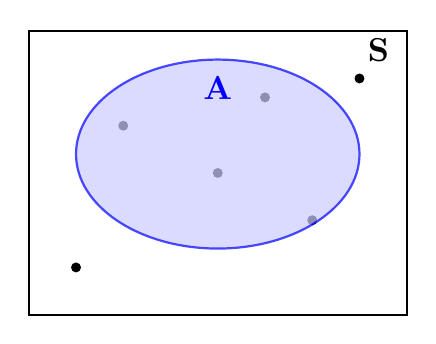
\begin{tikzpicture}[scale=1.2, every node/.style={transform shape}]
                    % Sample Space
                    \draw[thick] (-2,-1.5) rectangle (2,1.5);
                    \node at (1.7, 1.3) {\textbf{S}};
                    
                    % Elements/Outcomes
                    \fill (0,0) circle (1.5pt); \fill (-1,0.5) circle (1.5pt);
                    \fill (1,-0.5) circle (1.5pt); \fill (1.5,1) circle (1.5pt);
                    \fill (-1.5,-1) circle (1.5pt); \fill (0.5,0.8) circle (1.5pt);
                    
                    % Event A
                    \draw[thick, blue, fill=blue!20, opacity=0.7] (0,0.2) ellipse (1.5cm and 1cm);
                    \node[blue] at (0, 0.9) {\textbf{A}};
                \end{tikzpicture}
            \end{block}
        \end{column}
    \end{columns}
\end{frame}

\begin{frame}
    \frametitle{Intersection}
    
    \begin{columns}[T]
        \begin{column}{0.5\textwidth}
            \begin{block}{Explanation}
                The intersection of two sets, denoted as \(A \cap B\), is the set of all outcomes that are members of \textbf{both} set $A$ \textbf{and} set $B$.
                \vspace{1cm}
                
                In other words, the intersection is the event where both A and B occur simultaneously.
            \end{block}
        \end{column}
        
        \begin{column}{0.5\textwidth}
            \begin{block}{Diagram: \(A \cap B\)}
                \centering
                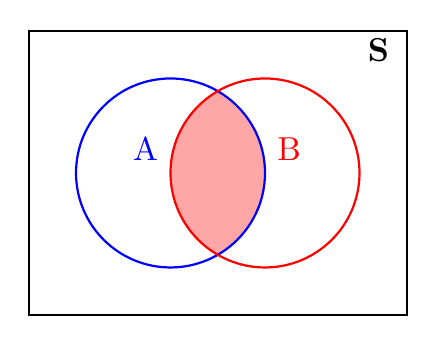
\begin{tikzpicture}[scale=1.2, every node/.style={transform shape}]
                    \draw[thick] (-2,-1.5) rectangle (2,1.5);
                    \node at (1.7, 1.3) {\textbf{S}};
                    
                    % Using scope for clipping
                    \begin{scope}
                        % Define the clipping path (circle A)
                        \clip (-0.5,0) circle (1cm);
                        % Fill circle B within the clipped area
                        \fill[red!50, opacity=0.7] (0.5,0) circle (1cm);
                    \end{scope}
                    
                    \draw[thick, blue] (-0.5,0) circle (1cm) node[above left] {A};
                    \draw[thick, red] (0.5,0) circle (1cm) node[above right] {B};
                \end{tikzpicture}
            \end{block}
        \end{column}
    \end{columns}
\end{frame}

\begin{frame}
    \frametitle{Union}
    
    \begin{columns}[T]
        \begin{column}{0.5\textwidth}
            \begin{block}{Explanation}
                The union of two sets, denoted as \(A \cup B\), is the set of all outcomes that are members of set $A$, \textbf{or} set $B$, \textbf{or} both.
                \vspace{1cm}
                
                In other words, the union is the event where at least one of A or B occurs.
            \end{block}
        \end{column}
        
        \begin{column}{0.5\textwidth}
            \begin{block}{Diagram: \(A \cup B\)}
                \centering
                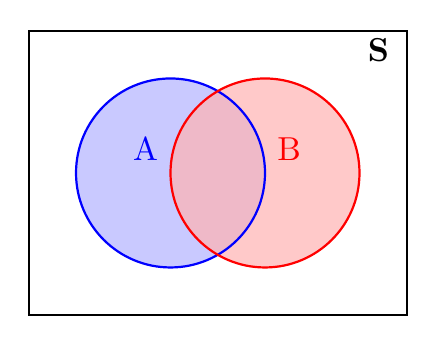
\begin{tikzpicture}[scale=1.2, every node/.style={transform shape}]
                    \draw[thick] (-2,-1.5) rectangle (2,1.5);
                    \node at (1.7, 1.3) {\textbf{S}};
                    
                    \fill[blue!30, opacity=0.7] (-0.5,0) circle (1cm);
                    \fill[red!30, opacity=0.7] (0.5,0) circle (1cm);
                    
                    \draw[thick, blue] (-0.5,0) circle (1cm) node[above left] {A};
                    \draw[thick, red] (0.5,0) circle (1cm) node[above right] {B};
                \end{tikzpicture}
            \end{block}
        \end{column}
    \end{columns}
\end{frame}

\begin{frame}
    \frametitle{Subset}
    
    \begin{columns}[T]
        \begin{column}{0.5\textwidth}
            \begin{block}{Explanation}
                Event A is called a subset of event B, written \(A \subset B\), if all outcomes in A are also outcomes in B.
                \vspace{1cm}
                
                In other words, the occurrence of A \textbf{guarantees} the occurrence of B.
            \end{block}
        \end{column}
        
        \begin{column}{0.5\textwidth}
            \begin{block}{Diagram: \(A \subset B\)}
                \centering
                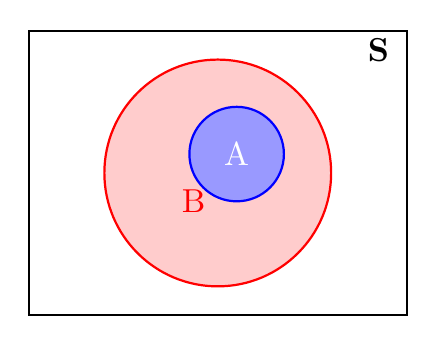
\begin{tikzpicture}[scale=1.2, every node/.style={transform shape}]
                    \draw[thick] (-2,-1.5) rectangle (2,1.5);
                    \node at (1.7, 1.3) {\textbf{S}};
                    
                    \draw[thick, red, fill=red!20] (0,0) circle (1.2cm) node [left,yshift=-0.3cm] {B};
                    \draw[thick, blue, fill=blue!40] (0.2,0.2) circle (0.5cm) node[white] {A};
                \end{tikzpicture}
            \end{block}
        \end{column}
    \end{columns}
\end{frame}

\begin{frame}
    \frametitle{Complement}
    
    \begin{columns}[T]
        \begin{column}{0.5\textwidth}
            \begin{block}{Explanation}
                The complement of a set $A$, denoted as \(A^c\), is the set of all outcomes in the universal set $S$ that are \textbf{not} members of set $A$.
                \vspace{1cm}
                
                In other words, the complement is the event that A does \textbf{not} occur.
            \end{block}
        \end{column}
        
        \begin{column}{0.5\textwidth}
            \begin{block}{Diagram: \(A^c\)}
                \centering
                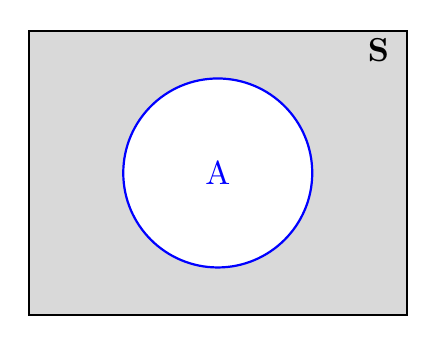
\begin{tikzpicture}[scale=1.2, every node/.style={transform shape}]
                    % Using even-odd rule to fill the area outside the circle
                    \fill[gray!30, even odd rule] (-2,-1.5) rectangle (2,1.5) (0,0) circle (1cm);
                    
                    \draw[thick] (-2,-1.5) rectangle (2,1.5);
                    \node at (1.7, 1.3) {\textbf{S}};
                    
                    \draw[thick, blue] (0,0) circle (1cm) node {A};
                \end{tikzpicture}
            \end{block}
        \end{column}
    \end{columns}
\end{frame}

\begin{frame}
    \frametitle{Mutually Exclusive}
    
    \begin{columns}[T]
        \begin{column}{0.5\textwidth}
            \begin{block}{Explanation}
                Two sets $A$ and $B$ are said to be mutually exclusive if they \textbf{cannot occur at the same time}.
                \vspace{1cm}
                
                This means their intersection is the empty set (\(A \cap B = \emptyset\)). Their Venn diagrams will not overlap.
            \end{block}
        \end{column}
        
        \begin{column}{0.5\textwidth}
            \begin{block}{Diagram: \(A \cap B = \emptyset \)}
                \centering
                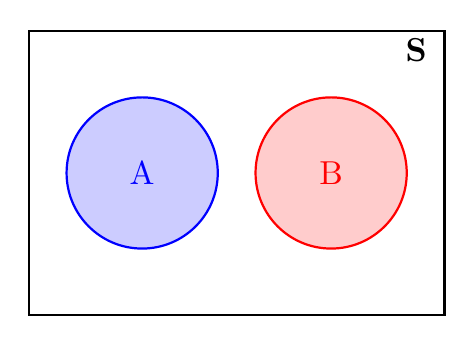
\begin{tikzpicture}[scale=1.2, every node/.style={transform shape}]
                    \draw[thick] (-2.2,-1.5) rectangle (2.2,1.5);
                    \node at (1.9, 1.3) {\textbf{S}};
                    
                    \draw[thick, blue, fill=blue!20] (-1,0) circle (0.8cm) node {A};
                    \draw[thick, red, fill=red!20] (1,0) circle (0.8cm) node {B};
                \end{tikzpicture}
            \end{block}
        \end{column}
    \end{columns}
\end{frame}

\begin{frame}
    \frametitle{Collectively Exhaustive}
    
    \begin{columns}[T]
        \begin{column}{0.5\textwidth}
            \begin{block}{Explanation}
                A collection of sets is said to be collectively exhaustive if their union \textbf{covers the entire} universal set (\(A \cup B = S\)).
                \vspace{1cm}
                
                Important: These sets are \textbf{not necessarily} mutually exclusive. If they overlap (as in the diagram), they do not form a partition.
            \end{block}
        \end{column}
        
        \begin{column}{0.5\textwidth}
            \begin{block}{Diagram: \(A \cup B=S\)}
                \centering
                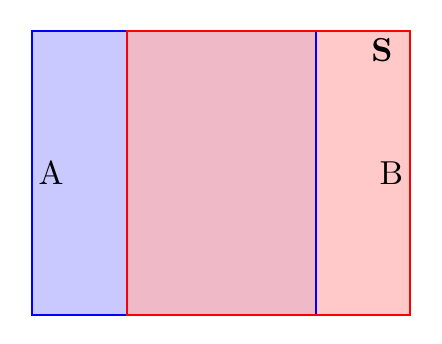
\begin{tikzpicture}[scale=1.2, every node/.style={transform shape}]
                    \begin{scope}
                        \clip (-2,-1.5) rectangle (2,1.5);
                        \fill[blue!30, opacity=0.7] (-2,-1.5) rectangle (1,1.5);
                        \fill[red!30, opacity=0.7] (-1,-1.5) rectangle (2,1.5);
                    \end{scope}
                    
                    \draw[thick] (-2,-1.5) rectangle (2,1.5);
                    \node at (1.7, 1.3) {\textbf{S}};
                    
                    \draw[thick, blue] (-2,-1.5) rectangle (1,1.5);
                    \node at (-1.8,0) {A};
                    \draw[thick, red] (-1,-1.5) rectangle (2,1.5);
                    \node at (1.8,0) {B};
                \end{tikzpicture}
            \end{block}
        \end{column}
    \end{columns}
\end{frame}

\begin{frame}
    \frametitle{Partition}
    
    \begin{columns}[T]
        \begin{column}{0.5\textwidth}
            \begin{block}{Explanation}
                A collection of sets \(\{B_1, B_2, ..., B_n\}\) is called a partition of the universal set $S$ if it meets two conditions:
                \begin{enumerate}
                    \item The sets are \textbf{mutually exclusive} (\(B_i \cap B_j = \emptyset\) for \(i \neq j\)).
                    \item The sets are \textbf{collectively exhaustive} (\(B_1 \cup B_2 \cup ... \cup B_n = S\)).
                \end{enumerate}
            \end{block}
        \end{column}
        
        \begin{column}{0.5\textwidth}
            \begin{block}{Diagram: \(S=\{B_1,B_2,B_3\}\)}
                \centering
                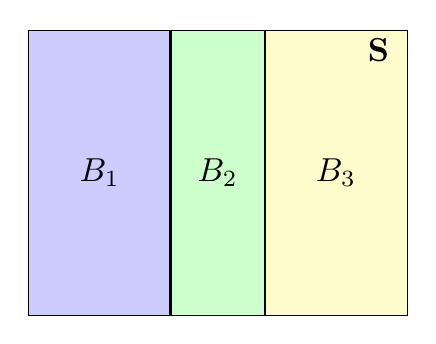
\begin{tikzpicture}[scale=1.2, every node/.style={transform shape}]
                    \draw[thick] (-2,-1.5) rectangle (2,1.5);
                    
                    \fill[blue!20] (-2,-1.5) rectangle (-0.5,1.5);
                    \fill[green!20] (-0.5,-1.5) rectangle (0.5,1.5);
                    \fill[yellow!20] (0.5,-1.5) rectangle (2,1.5);
                    
                    \draw[thick] (-0.5, -1.5) -- (-0.5, 1.5);
                    \draw[thick] (0.5, -1.5) -- (0.5, 1.5);
                    
                    \node at (-1.25, 0) {\(B_1\)};
                    \node at (0, 0) {\(B_2\)};
                    \node at (1.25, 0) {\(B_3\)};
                    \node at (1.7, 1.3) {\textbf{S}};
                \end{tikzpicture}
            \end{block}
        \end{column}
    \end{columns}
\end{frame}

\begin{frame}[t]
\frametitle{\ }
\begin{columns}[T]
    % Column for Set Operations
    \begin{column}{0.5\textwidth}
        \begin{block}{Set Operations}
            \begin{itemize}
                \item \textbf{Intersection:} $A \cap B$ \\ The set where \textbf{A AND B} both occur.
                \item \textbf{Union:} $A \cup B$ \\ The set where \textbf{A OR B} (or both) occur.
                \item \textbf{Complement:} $A^c$ \\ The set where \textbf{NOT A} occurs.
            \end{itemize}
        \end{block}
    \end{column}
    
    % Column for Boolean Logic
    \begin{column}{0.5\textwidth}
        \begin{block}{Boolean Operations}
            \begin{itemize}
                \item \textbf{Logical AND} \\ The output is TRUE if all statements are true.
                \item \textbf{Logical OR} \\ The output is TRUE if at least one statement is true.
                \item \textbf{Logical NOT} \\ The output is TRUE if the statement is false.
            \end{itemize}
        \end{block}
    \end{column}
\end{columns}
\end{frame}

% --- NEW SLIDE: De Morgan's Law ---
\begin{frame}
    \frametitle{\ }
    \vspace{-9mm}
    \begin{columns}[T]
        \begin{column}{0.5\textwidth}
            \begin{Teorema}[De Morgan's Law]
                \[ (A \cap B)^c = A^c \cup B^c \]
            \end{Teorema}
            
            \begin{block}{Diagram Explanation}
                De Morgan's Law states that the complement of the intersection of two sets is the same as the union of their complements.
                \vspace{0.5cm}
                
                Visually, the area outside the intersection \(A \cap B\) (the shaded area) is the same as the union of the area outside A and the area outside B.
            \end{block}
        \end{column}
        
        \begin{column}{0.5\textwidth}
            \begin{block}{Diagram: \((A \cap B)^c = A^c \cup B^c\)}
                \centering
                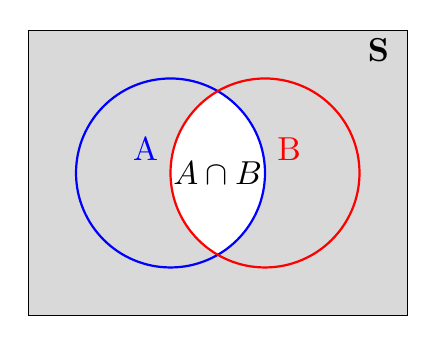
\begin{tikzpicture}[scale=1.2, every node/.style={transform shape}]
                    \draw[thick] (-2,-1.5) rectangle (2,1.5);
                    
                    % Shade the entire area S
                    \fill[gray!30] (-2,-1.5) rectangle (2,1.5);
                    
                    % "Erase" the shading in the intersection area with white
                    \begin{scope}
                        \clip (-0.5,0) circle (1cm);
                        \fill[white] (0.5,0) circle (1cm);
                    \end{scope}
                    
                    % Redraw the outlines to be visible
                    \draw[thick, blue] (-0.5,0) circle (1cm) node[above left] {A};
                    \draw[thick, red] (0.5,0) circle (1cm) node[above right] {B};
                    \node at (1.7, 1.3) {\textbf{S}};
                    \node at (0, 0) {\(A \cap B\)};
                \end{tikzpicture}
            \end{block}
        \end{column}
    \end{columns}
\end{frame}

\subsubsection{Probability and Related Terms}
\begin{frame} \vfill \centering \begin{beamercolorbox}[sep=10pt,center,shadow=false,rounded=true]{section_begin} \usebeamerfont{section_begin}\insertsubsubsectionhead\par \end{beamercolorbox} \vfill \end{frame}

\begin{frame}[t]
\frametitle{\ }
\begin{table}[]
    \centering
    \caption{Equivalence of Concepts: Probability Theory vs. Set Theory}
    \label{tab:placeholder}
    \begin{tabular}{cc}
    \hline
        \textbf{Set Theory} & \textbf{Probability Theory} \\
    \hline
        Set & Event \\
        Universal Space & Sample Space \\
        Element & Outcome \\
        \hline
    \end{tabular}
\end{table}
\end{frame}

\begin{frame}[t]
\frametitle{\ }
\vspace{-7.5mm}
\begin{Definisi}[Probability and Related Terms (\only<1>{1}\only<2>{2}/2)]
    \begin{itemize}
    \only<1>{
        \item \textbf{Outcome:} Any possible result of an observation process obtained from an experiment. Example: a specific keyword is not present in a comment; a comment is \textit{spam} / \textit{ham}.
        \item \textbf{Event:} A set of outcomes from an experiment. Example: Event $A$ = the set of all \textit{spam} comments.
        \item \textbf{Sample Space ($S$):} The set of all possible outcomes, where the outcomes are mutually exclusive. Example: $S$ is all existing comments; the class of a comment is \textit{spam} / \textit{ham}.
        }
        \only<2>{
        \item \textbf{Experiment:} A sequence of procedures performed systematically, accompanied by an observation process. Example: counting a specific keyword in a social media comment; classifying a comment as \textit{spam} / \textit{ham}.
        \item \textbf{Outcome:} Any possible result of an observation process obtained from an experiment. Example: a specific keyword is not present in a comment; a comment is \textit{spam} / \textit{ham}.
        \item \textbf{Probability:} A measure that describes the likelihood of an outcome or event occurring as a result of a repeated experiment.
        }
    \end{itemize}
\end{Definisi}
\end{frame}

\subsubsection{Axioms of Probability}
\begin{frame} \vfill \centering \begin{beamercolorbox}[sep=10pt,center,shadow=false,rounded=true]{section_begin} \usebeamerfont{section_begin}\insertsubsubsectionhead\par \end{beamercolorbox} \vfill \end{frame}

\begin{frame}[t,fragile]
\frametitle{\ }
\vspace{-5mm}
\setbeamertemplate{enumerate items}[default]
\begin{Aksioma}[The Basic Rules of Probability]
    Every probability theory is built upon three basic rules (axioms):
    \begin{enumerate}
        \only<1->{
        \item For any event $A$, its probability is non-negative: $P(A) \ge 0$.
        }
        \only<2->{
        \item The probability of the entire sample space $S$ is 1: $P(S) = 1$.
        }
        \only<3->{
        \item For mutually exclusive events ($A_1, A_2, \dots$), the probability of their union is the sum of their individual probabilities: $P(A_1 \cup A_2 \cup \dots) = P(A_1) + P(A_2) + \dots$.
        }
    \end{enumerate}
\end{Aksioma}

\vspace{-1em}

\only<1>{
    \begin{block}{}
    \justifying
        Probability cannot be negative. Its smallest value is 0, which means an event is impossible. Example: the probability of rolling a 7 on a standard six-sided die is 0.
    \end{block}
}
\only<2>{
    \begin{block}{}
    \justifying
        If we conduct an experiment, one of all possible outcomes is \textbf{certain} to occur. The probability of a certainty is 1. \textbf{Example}: the probability of rolling a number between 1 and 6 on a die is 1.
    \end{block}
}
\only<3>{
    \begin{block}{}
    \justifying
        If two events cannot happen at the same time (mutually exclusive), the probability that one of them occurs is simply the sum of their individual probabilities. \textbf{Example}: $P(\text{roll a 1 or 2}) = P(\text{roll a 1}) + P(\text{roll a 2})$.
    \end{block}
}
\end{frame}

\subsubsection{Theorems for Mutually Exclusive Events}
\begin{frame}[t]
\frametitle{\ }
    \begin{block}{Elaboration on Axiom 3}
    \begin{itemize}
        \item One point from the axioms that needs attention is how we define and calculate the probability of mutually exclusive events.
        \item We will elaborate on 2 additional theorems to discuss this third axiom.
    \end{itemize}
    \end{block}
\end{frame}

\begin{frame}[t]
\frametitle{\ }
  \vspace{-8mm}
  \footnotesize
  \begin{Teorema}[Probability of the Union of Two Mutually Exclusive Events]
    For two mutually exclusive events $A_1$ and $A_2$, the probability of their union is the sum of their individual probabilities.
    \[
      P(A_1 \cup A_2) = P(A_1) + P(A_2)
    \]
  \end{Teorema}
  
  \vfill % Vertical space
  \vspace{-5mm}
  \begin{block}{}
  \justifying
    Imagine two things that \textbf{cannot happen at the same time}. For example, in a single coin toss, you cannot get both "Heads" and "Tails".
    
    This theorem states that to find the probability of \textbf{either} of these two events occurring, you simply \textbf{add} their individual probabilities.
    
    \medskip % Small vertical space
    
    \textbf{Example:} The probability of rolling a 1 on a die is 1/6. The probability of rolling a 2 is also 1/6. Since you cannot roll a 1 and a 2 at the same time, the probability of rolling a 1 \textit{or} a 2 is $1/6 + 1/6 = 2/6$.
  \end{block}
  
\end{frame}

\begin{frame}[t]
\frametitle{\ }
  \vspace{-8mm}
  \footnotesize
  \begin{Teorema}[Probability of the Union of Many Mutually Exclusive Events]
    If an event $A$ can be broken down into $m$ mutually exclusive "pieces" ($A_1, A_2, \dots, A_m$), then the probability of event $A$ is the total sum of the probabilities of all its "pieces".
    \[
      P(A) = \sum_{i=1}^{m} P(A_i)
    \]
  \end{Teorema}
  
  \vfill
  \vspace{-5mm}
  \begin{block}{}
    This is a more advanced version of the first theorem, applicable to \textbf{many events}, not just two. Think of a "large event" composed of several non-overlapping "small events". This theorem says that the probability of the large event is equal to the \textbf{sum of the probabilities} of all its constituent small events.
    
    \medskip
    
    \textbf{Example:} The event "rolling an even number" on a die (this is the large event $A$). This event can be broken into 3 mutually exclusive pieces: \{rolling a 2\}, \{rolling a 4\}, and \{rolling a 6\}. Thus, the probability of rolling an even number is:
    $P(\text{even}) = P(2) + P(4) + P(6) = 1/6 + 1/6 + 1/6 = 3/6$.
  \end{block}
  
\end{frame}

\begin{frame}
    \frametitle{Property of Probability: Union of Mutually Exclusive Events}
\footnotesize
    \vspace{-3mm}
    \begin{columns}[T]
        \begin{column}{0.5\textwidth}
            \begin{block}{Theorem}
                If an event $A$ can be decomposed into $m$ mutually exclusive "pieces" ($A_1, \dots, A_m$), then the probability of $A$ is the sum of the probabilities of all its pieces.
                \[ P(A) = \sum_{i=1}^{m} P(A_i) \]
            \end{block}
            \vspace{-4mm}
            \begin{block}{Diagram Explanation}
                The total area of event A (the colored area) is the sum of the areas of its constituent pieces (\(A_1, A_2, A_3\)).
            \end{block}
        \end{column}
        
        \begin{column}{0.5\textwidth}
            \begin{block}{Diagram}
                \centering
                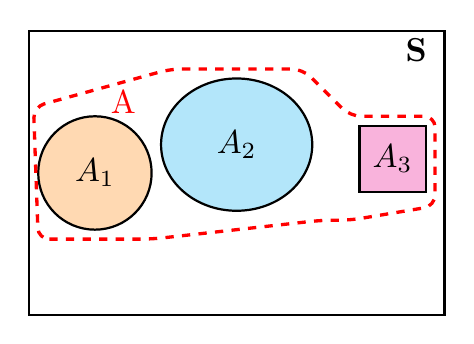
\begin{tikzpicture}[scale=1.2, every node/.style={transform shape}]
                    \draw[thick] (-2.2,-1.5) rectangle (2.2,1.5);
                    \node at (1.9, 1.3) {\textbf{S}};
                    
                    % Draw event A as the union of A1, A2, A3
                    \draw[thick, fill=orange!30] (-1.5,0) circle (0.6cm);
                    \node at (-1.5,0) {\(A_1\)};
                    
                    \draw[thick, fill=cyan!30] (0,0.3) ellipse (0.8cm and 0.7cm);
                    \node at (0,0.3) {\(A_2\)};
                    
                    \draw[thick, fill=magenta!30] (1.3,-0.2) rectangle (2,0.5);
                    \node at (1.65,0.15) {\(A_3\)};
                    
                    % Outline for A
                    \draw[very thick, red, dashed, rounded corners] (-2.1, -0.7) -- (-0.9,-0.7) -- (0.9,-0.5) -- (1.2,-0.5) -- (2.1,-0.35) -- (2.1,0.6) -- (1.2,0.6) -- (0.7,1.1) -- (-0.7,1.1) -- (-2.15,0.7) -- cycle;
                    \node[red] at (-1.2,0.75) {A};
                    
                \end{tikzpicture}
            \end{block}
        \end{column}
    \end{columns}
\end{frame}

\subsubsection{Theorems on Properties of Probability}
\begin{frame} \vfill \centering \begin{beamercolorbox}[sep=10pt,center,shadow=false,rounded=true]{section_begin} \usebeamerfont{section_begin}\insertsubsubsectionhead\par \end{beamercolorbox} \vfill \end{frame}

\begin{frame}[t]
\frametitle{\ }
    \begin{block}{Implications of the Probability Axioms}
        Using the axioms of probability, we can also derive theorems about the basic properties of probability.
    \end{block}
\end{frame}

\begin{frame}[t,fragile]
\frametitle{\ }
\vspace{-5mm}
\setbeamertemplate{enumerate items}[default]
\begin{Teorema}[Properties of Probability]
    As a consequence of the three axioms, we can prove the following theorems:
    \begin{enumerate}
        \only<1->{
        \item The probability of an impossible event is zero: $P(\emptyset) = 0$.
        }
        \only<2->{
        \item The probability of the complement of an event: $P(A^c) = 1 - P(A)$.
        }
        \only<3->{
        \item The addition rule for two events: $P(A \cup B) = P(A) + P(B) - P(A \cap B)$.
        }
        \only<4->{
        \item If $A \subset B$, then $P(A) \le P(B)$.
        }
    \end{enumerate}
\end{Teorema}

\vspace{-1em}

\only<1>{
    \begin{block}{}
    \justifying
        This is the logical inverse of certainty. If the probability of the entire sample space (an event that is certain to happen) is 1, then the probability of the empty set (an impossible event) is 0. \textbf{Example}: The probability of rolling an 8 on a six-sided die is 0.
    \end{block}
}
\only<2>{
    \begin{block}{}
    \justifying
        The probability that an event will \textbf{not} happen is 1 minus the probability that it will. Here, $A^c$ (read: A complement) includes all possible outcomes not in A. \textbf{Example}: If the probability of rain tomorrow is 40\% ($P(A)=0.4$), then the probability of no rain tomorrow is $1 - 0.4 = 0.6$ or 60\%.
    \end{block}
}
\only<3>{
    \begin{block}{}
    \justifying
        To find the probability of the union of two events that \textit{can} happen together, we add their individual probabilities, then subtract the probability of them both happening together. This subtraction is done \textbf{so that the intersection ($A \cap B$) is not counted twice}.
    \end{block}
}
\only<4>{
    \begin{block}{}
    \justifying
       If event A is a subset of event B (meaning every outcome in A is also in B), then the probability of A can never be greater than B. \textbf{Example}: The event "getting the King of Hearts" ($A$) is a subset of the event "getting a Hearts card" ($B$). Naturally, $P(A) = 1/52$ is less than $P(B) = 13/52$.
    \end{block}
}
\end{frame}

% --- NEW SLIDE 1: Property of Probability 1 ---
\begin{frame}
    \frametitle{Properties of Probability (1)}
    \footnotesize
    \begin{columns}[T]
        \begin{column}{0.5\textwidth}
            \begin{block}{Theorem 1: Probability of a Complement}
                \[ P(A^c) = 1 - P(A) \]
            \end{block}
            
            \begin{block}{Diagram Explanation}
                An event A and its complement \(A^c\) form a partition of the sample space S. They are mutually exclusive, and their union is S.
                \vspace{0.5cm}
                
                Since \(P(S)=1\), it follows that \(P(A) + P(A^c) = 1\). Thus, the probability of \(A^c\) (the gray area) is 1 minus the probability of A (the blue area).
            \end{block}
        \end{column}
        
        \begin{column}{0.5\textwidth}
            \begin{block}{Diagram}
                \centering
                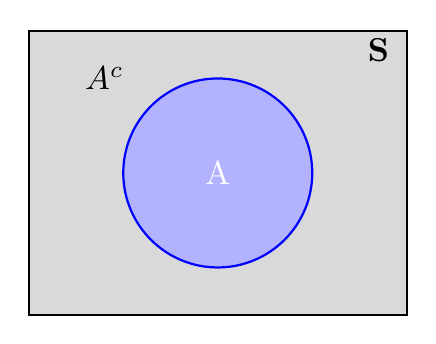
\begin{tikzpicture}[scale=1.2, every node/.style={transform shape}]
                    \fill[gray!30] (-2,-1.5) rectangle (2,1.5);
                    \fill[blue!30] (0,0) circle (1cm);
                    
                    \draw[thick] (-2,-1.5) rectangle (2,1.5);
                    \node at (1.7, 1.3) {\textbf{S}};
                    
                    \draw[thick, blue] (0,0) circle (1cm) node[white] {A};
                    \node at (-1.2, 1) {\(A^c\)};
                \end{tikzpicture}
            \end{block}
        \end{column}
    \end{columns}
\end{frame}

% --- NEW SLIDE 2: Property of Probability 2 ---
\begin{frame}
    \frametitle{Properties of Probability (2)}
    \footnotesize
    \begin{columns}[T]
        \begin{column}{0.5\textwidth}
            \begin{block}{Theorem 2: The Addition Rule}
                \[ P(A \cup B) = P(A) + P(B) - P(A \cap B) \]
            \end{block}
            
            \begin{block}{Diagram Explanation}
                If we add the area of A and the area of B directly, the intersection area (\(A \cap B\)) will be counted \textbf{twice}.
                \vspace{0.5cm}
                
                Therefore, to get the correct total union area, we must subtract the double-counted intersection area one time.
            \end{block}
        \end{column}
        
        \begin{column}{0.5\textwidth}
            \begin{block}{Diagram}
                \centering
                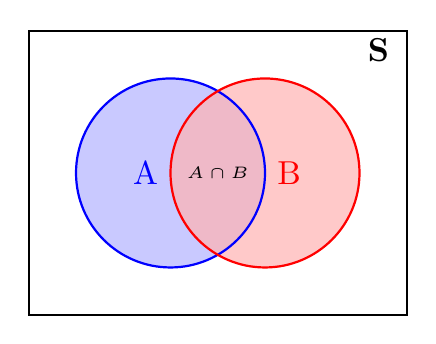
\begin{tikzpicture}[scale=1.2, every node/.style={transform shape}]
                    \draw[thick] (-2,-1.5) rectangle (2,1.5);
                    \node at (1.7, 1.3) {\textbf{S}};
                    
                    \fill[blue!30, opacity=0.7] (-0.5,0) circle (1cm);
                    \fill[red!30, opacity=0.7] (0.5,0) circle (1cm);
                    
                    \draw[thick, blue] (-0.5,0) circle (1cm) node[left] {A};
                    \draw[thick, red] (0.5,0) circle (1cm) node[right] {B};
                    
                    \node at (0,0) {\tiny \(A \cap B\)};
                \end{tikzpicture}
            \end{block}
        \end{column}
    \end{columns}
\end{frame}

% --- NEW SLIDE 3: Property of Probability 3 ---
\begin{frame}
    \frametitle{Properties of Probability (3)}
    \footnotesize
    \begin{columns}[T]
        \begin{column}{0.5\textwidth}
            \begin{block}{Theorem 3: Subset Events}
                If \(A \subset B\), then \(P(A) \le P(B)\).
            \end{block}
            
            \begin{block}{Diagram Explanation}
                If A is a subset of B, then the entire area of A is \textbf{inside} the area of B.
                \vspace{0.5cm}
                
                Visually, it is impossible for the area of A (the part) to be larger than the area of B (the whole). Therefore, the probability of A must be less than or equal to the probability of B.
            \end{block}
        \end{column}
        
        \begin{column}{0.5\textwidth}
            \begin{block}{Diagram}
                \centering
                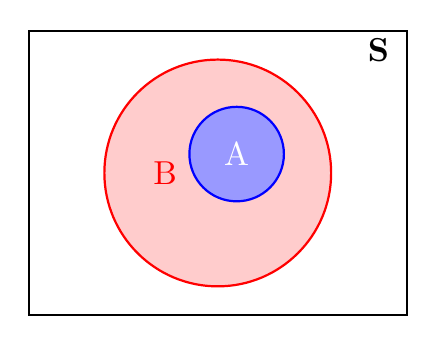
\begin{tikzpicture}[scale=1.2, every node/.style={transform shape}]
                    \draw[thick] (-2,-1.5) rectangle (2,1.5);
                    \node at (1.7, 1.3) {\textbf{S}};
                    
                    \draw[thick, red, fill=red!20] (0,0) circle (1.2cm) node [left,xshift=-0.3cm]{B};
                    \draw[thick, blue, fill=blue!40] (0.2,0.2) circle (0.5cm) node[white] {A};
                \end{tikzpicture}
            \end{block}
        \end{column}
    \end{columns}
\end{frame}

\begin{frame}[t]
\frametitle{\ }
  \vspace{-8mm}
  \footnotesize
  \begin{Teorema}[Probability of an Event from its Outcomes]
    The probability of an event $B$, which consists of the set of basic outcomes $\{s_1, s_2, \dots, s_m\}$, is the sum of the probabilities of each basic outcome contained within it.
    \[
      P(B) = \sum_{i=1}^{m} P(\{s_i\})
    \]
  \end{Teorema}
  
  \vfill
  \vspace{-5mm}

    \begin{block}{}
    This theorem formalizes the most basic way of calculating probability. It distinguishes between an "outcome" and an "event".
    \begin{itemize}
        \item \textbf{Outcome:} A single, most basic possible result. Example: Getting \textit{exactly} a 5 on a die roll.
        \item \textbf{Event:} A \textit{collection} of one or more outcomes. Example: "Getting an odd number" on a die roll.
    \end{itemize}
    
    This theorem states: to find the probability of an \textbf{event}, simply \textbf{sum the probabilities of all the basic outcomes} that make up that event.
  \end{block}
  
\end{frame}

\subsubsection{Probability Notation Conventions}
\begin{frame} \vfill \centering \begin{beamercolorbox}[sep=10pt,center,shadow=false,rounded=true]{section_begin} \usebeamerfont{section_begin}\insertsubsubsectionhead\par \end{beamercolorbox} \vfill \end{frame}
\begin{frame}[t]
\frametitle{\ }
\begin{alertblock}{Probability Notation}
    Let's take a moment to agree on the probability notation conventions we will use throughout this course.
\end{alertblock}    
\end{frame}

\begin{frame}[t]
\frametitle{\ }
\vspace{-8mm}

\only<1>{
  \begin{block}{Basic Notation: P[ ]}
    The notation $\textbf{P}[A]$ is used to denote the \textbf{probability of the event $A$}.
    \begin{itemize}
        \item Inside the square brackets $[\,]$ is an \textbf{event}, which is fundamentally a \textbf{set}.
        \item The function $P[\cdot]$ maps an event to a number between $0$ and $1$.
    \end{itemize}
  \end{block}
}
\only<2>{
  \begin{block}{Single Outcome Notation}
    Formally, a basic outcome $s_i$ must be written as a set $\{s_i\}$ when placed inside the probability notation.
    \begin{itemize}
        \item Formal Notation: $P[\{s_i\}]$ $\rightarrow$ the probability of the event containing only the single outcome $s_i$.
        \item \textbf{Shorthand Notation:} For practicality, it is often written more concisely as $P[s_i]$. Both have the same meaning.
    \end{itemize}
  \end{block}
}
\only<3>{
  \begin{alertblock}{Intersection Notation}
    The probability of the intersection of two events $A$ and $B$ (i.e., the event where $A$ \textbf{and} $B$ both occur) has several equivalent notations:
    \begin{itemize}
        \item Formal Notation: $P[A \cap B]$
        \item Alternative Notation: $P[A, B]$
        \item Most Concise Notation: $P[AB]$
    \end{itemize}
    These three notations mean the same thing and can be used interchangeably.
  \end{alertblock}
}
\end{frame}

\subsubsection{Equally Likely Outcomes}
\begin{frame} \vfill \centering \begin{beamercolorbox}[sep=10pt,center,shadow=false,rounded=true]{section_begin} \usebeamerfont{section_begin}\insertsubsubsectionhead\par \end{beamercolorbox} \vfill \end{frame}
\begin{frame}[t]
\frametitle{\ }
\footnotesize
\vspace{-7mm}
  \begin{block}{Intuitive Concept}
    In many real-world experiments, we have a basic assumption that every possible outcome has the \textbf{exact same chance} of occurring. This is usually based on the symmetry or "fairness" of the experiment.
    \begin{itemize}
        \item \textbf{Fair Coin:} The chance of getting "Heads" is the same as the chance of "Tails".
        \item \textbf{Balanced Die:} The chance of any side (1, 2, 3, 4, 5, or 6) appearing is the same.
        \item \textbf{Playing Cards:} The chance of drawing any specific card from a well-shuffled deck is the same.
    \end{itemize}
    This concept is the foundation of the simplest probability models.
  \end{block}
\end{frame}

\begin{frame}[t]
\frametitle{\ }
\setbeamertemplate{enumerate items}[default]
\vspace{-7mm}
\footnotesize
  \begin{Teorema}[Probability of Equally Likely Outcomes]
    For an experiment with a sample space $S = \{s_1, s_2, \dots, s_n\}$ containing $n$ outcomes, where each outcome has an equal chance of occurring, the probability of any single outcome $s_i$ is:
    \[
      P[s_i] = \frac{1}{n}
    \]
  \end{Teorema}
  \vspace{-1mm}
  \vspace{-3mm}
  \begin{alertblock}{}
    This formula comes directly from two basic principles:
    \begin{enumerate}
        \item \textbf{Assumption of Equal Probability:} Let's call the probability of any outcome $p$. So, $P[s_1] = p$, $P[s_2] = p$, ..., $P[s_n] = p$.
        \item \textbf{Axiom of Total Probability:} The total probability of all possible outcomes in an experiment \textbf{must equal 1}.
    \end{enumerate}
    By combining these two, the total probability is the sum of the probabilities of all outcomes: $p + p + \dots + p$ ($n$ times). This means $\mathbf{n \times p = 1}$.
    
    From this simple equation, we can directly conclude that $\mathbf{p = 1/n}$.
  \end{alertblock}
\end{frame}

\subsubsection{Conditional Probability}
\begin{frame} \vfill \centering \begin{beamercolorbox}[sep=10pt,center,shadow=false,rounded=true]{section_begin} \usebeamerfont{section_begin}\insertsubsubsectionhead\par \end{beamercolorbox} \vfill \end{frame}
\begin{frame}[t]
\frametitle{\ }
\vspace{-8mm}
\footnotesize
\begin{Definisi}[Conditional Probability]
    The probability of event A \textit{given that} event B has occurred.
    \[ P(A|B) = \frac{P(A \cap B)}{P(B)} \]
\end{Definisi}
\vspace{-3mm}
\begin{block}{Example Question}
Suppose you draw one card at random from a standard 52-card deck. Let event B be that the card drawn is Red, and event A is that the card drawn is a Queen. What does \( P(A|B) \) mean?
\end{block}
\begin{exampleblock}{Solution}
\( P(A|B) \) means: "What is the probability that the card is a \textbf{Queen}, \textbf{given that we already know} the card is \textbf{Red}?"

\vspace{0.5mm}
\textbf{Explanation:}
Since we already know the card is Red (event B has occurred), our sample space is no longer 52 cards, but only the 26 red cards. Of those 26 red cards, there are 2 Queens (the Queen of Hearts and the Queen of Diamonds). So, the probability is 2 out of 26, or \( \frac{2}{26} = \frac{1}{13} \).
\end{exampleblock}
\end{frame}

\begin{frame}
    \frametitle{\ }
    \vspace{-7mm}
    \footnotesize
    \begin{columns}[T]
        \begin{column}{0.5\textwidth}
            \begin{block}{Definition}
                The probability of event A \textit{given that} event B has occurred.
                \[ P(A|B) = \frac{P(A \cap B)}{P(B)} \]
            \end{block}
            
            \begin{block}{Diagram Explanation}
            \only<1>{
                Initially, our effective sample space is S.
                \vspace{0.5cm}
                
                The probability of A occurring in this condition is the area of \(A\) divided by the total area of S = \(P(A)\).
                }
            \only<2>{
                When we know that event \textbf{B} has occurred, our effective sample space shrinks from S to just B.
                \vspace{0.5cm}
                
                The probability of A occurring in this new condition is the proportion of B that is also part of A, which is the intersection area \(A \cap B\) divided by the total area of B = \(P(A|B)\).
                }
            \end{block}
        \end{column}
        
        \begin{column}{0.5\textwidth}
            \begin{block}{Diagram: \only<1>{S is the Original Sample Space}\only<2>{B is the New Sample Space}}
                \centering
                \begin{tikzpicture}[scale=1.2, every node/.style={transform shape}]
                    \draw[thick] (-2,-1.5) rectangle (2,1.5);
                    \node at (1.7, 1.3) {\textbf{S}};

                    \only<1>{
                    % Color S as the old sample space
                    \fill[yellow!40](-2,-1.5) rectangle (2,1.5);
                    }
                    \only<2>{
                    % Color B as the new sample space
                    \fill[yellow!40] (0.5,0) circle (1cm);
                    }

                    \only<1>{     \fill[orange!80] (-0.5,0) circle (1cm);
                    }
                    \only<2>{
                    % Use clip to color the intersection on top of B
                    \begin{scope}
                        \clip (0.5,0) circle (1cm);
                        \fill[orange!80] (-0.5,0) circle (1cm);
                    \end{scope}
                    }
                    % Draw outlines
                    \draw[thick, blue] (-0.5,0) circle (1cm) node[above left] {A};
                    \draw[thick, red] (0.5,0) circle (1cm) node[above right] {B};
                    
                    % Labels
                    \only<1>{
                    \node[align=center] at (-0.9,0) {\tiny \(P(A)\)};
                    }
                    \only<2>{
                    \node[align=center] at (0.9,0) {\tiny \(P(B)\)};
                    \node[align=center] at (0,0) {\tiny \(P(A \cap B)\)};
                    }
                \end{tikzpicture}
            \end{block}
        \end{column}
    \end{columns}
\end{frame}

\begin{frame}[t]
\frametitle{\ }
\footnotesize
\vspace{-3mm}
    \begin{Teorema}[Properties of Conditional Probability]
        \begin{description}
            \item[Axiom 1] $P[A|B] \ge 0$. \textit{\footnotesize (Conditional probability is never negative.)}
            \only<2->{
            \item[Axiom 2] $P[B|B] = 1$. \textit{\footnotesize (The probability of B happening, given we know B happened, is a certainty.)}
            }
            \only<3->{
            \item [Axiom 3] If $A = A_1 \cup A_2 \cup \dots$ with $A_i \cap A_j = \emptyset$ for $i \neq j$, then
            \[ P[A|B] = P[A_1|B] + P[A_2|B] + \dots \]
            \textit{(The addition rule also applies to conditional probability.)}
            }
        \end{description}
    \end{Teorema}
    \only<1>{
    \begin{block}{}
    \textbf{Example:} Draw a ball from a bag (5R, 3B, 2G). Given the ball is not Green (event B), the probability of getting Blue (event A) is $P[A|B] = 3/8 \ge 0$.
    \end{block}
    }
    \only<2>{
    \begin{block}{}
    \textbf{Example:} Roll a die. Given the result is even (B), the probability that the result is even is $P[B|B] = 1$.
    \end{block}
    }
    \only<3>{
    \begin{block}{}
    \textbf{Example:} Draw a card. Given the card is a face card (B). $$P[\text{King or Queen}|B] = P[\text{King}|B] + P[\text{Queen}|B] = \frac{4}{12} + \frac{4}{12} = \frac{8}{12}$$.
    \end{block}
    }
\end{frame}

% --- NEW SLIDE 1: Axiom 1 ---
\begin{frame}
    \frametitle{Properties of Conditional Probability: Axiom 1}
    
    \begin{columns}[T]
        \begin{column}{0.5\textwidth}
            \begin{block}{Axiom 1: \(P[A|B] \ge 0\)}
                Conditional probability is never negative.
            \end{block}
            
            \begin{block}{Diagram Explanation}
                The probabilities \(P(A \cap B)\) and \(P(B)\) are represented by the \textbf{area} in a Venn diagram. Since area cannot be negative, the result of their division (\(P(A|B)\)) also cannot be negative.
            \end{block}
        \end{column}
        
        \begin{column}{0.5\textwidth}
            \begin{block}{Diagram}
                \centering
                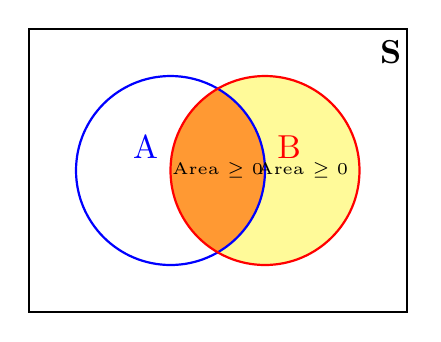
\begin{tikzpicture}[scale=1.2, every node/.style={transform shape}]
                    \draw[thick] (-2,-1.5) rectangle (2,1.5)node[below,xshift=-0.17cm]{\textbf{S}};
                    \fill[yellow!40] (0.5,0) circle (1cm);
                    \begin{scope}
                        \clip (0.5,0) circle (1cm);
                        \fill[orange!80] (-0.5,0) circle (1cm);
                    \end{scope}
                    \draw[thick, blue] (-0.5,0) circle (1cm) node[above left] {A};
                    \draw[thick, red] (0.5,0) circle (1cm) node[above right] {B};
                    \node at (0.9,0) {\tiny Area \(\ge 0\)};
                    \node at (0,0) {\tiny Area \(\ge 0\)};
                \end{tikzpicture}
            \end{block}
        \end{column}
    \end{columns}
\end{frame}

% --- NEW SLIDE 2: Axiom 2 ---
\begin{frame}
    \frametitle{Properties of Conditional Probability: Axiom 2}
    
    \begin{columns}[T]
        \begin{column}{0.5\textwidth}
            \begin{block}{Axiom 2: \(P[B|B] = 1\)}
                The probability of B occurring, given that we already know B has occurred, is a certainty.
            \end{block}
            
            \begin{block}{Diagram Explanation}
                If we are told that event B has occurred, then B becomes our new sample space. The probability of B occurring within this new sample space is 1 (or 100\%), because the entire sample space is B itself.
                \[ P(B|B) = \frac{P(B \cap B)}{P(B)} = \frac{P(B)}{P(B)} = 1 \]
            \end{block}
        \end{column}
        
        \begin{column}{0.5\textwidth}
            \begin{block}{Diagram}
                \centering
                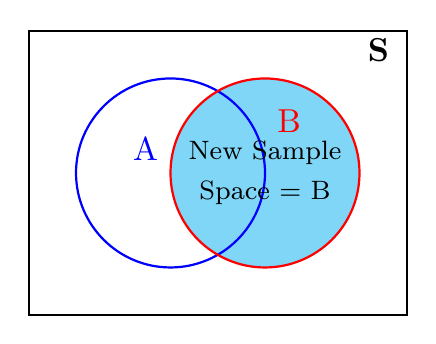
\begin{tikzpicture}[scale=1.2, every node/.style={transform shape}]
                    \draw[thick] (-2,-1.5) rectangle (2,1.5);
                    \node at (1.7, 1.3) {\textbf{S}};
                    
                    % Entire B is colored as the event and the new sample space
                    \fill[cyan!50] (0.5,0) circle (1cm);
                    
                    \draw[thick, blue] (-0.5,0) circle (1cm) node[above left] {A};
                    \draw[thick, red] (0.5,0) circle (1cm) node[above right,yshift=0.3cm] {B};
                    
                    \node[align=center] at (0.5,0) {\footnotesize New Sample \\ \footnotesize Space = B};
                \end{tikzpicture}
            \end{block}
        \end{column}
    \end{columns}
\end{frame}

% --- NEW SLIDE 3: Axiom 3 ---
\begin{frame}
    \frametitle{Properties of Conditional Probability: Axiom 3}
    
    \begin{columns}[T]
        \begin{column}{0.5\textwidth}
            \begin{block}{Axiom 3: The Addition Rule}
                If \(A_1\) and \(A_2\) are mutually exclusive, then:
                \[ P[A_1 \cup A_2 | B] = P[A_1|B] + P[A_2|B] \]
            \end{block}
            
            \begin{block}{Diagram Explanation}
                Within the new sample space B, the probability of being in the combined area (\(A_1 \cup A_2\)) is the sum of the probabilities of the respective intersection areas (\(P(A_1 \cap B)\) and \(P(A_2 \cap B)\)) divided by the probability of B.
            \end{block}
        \end{column}
        
        \begin{column}{0.5\textwidth}
            \begin{block}{Diagram}
                \centering
                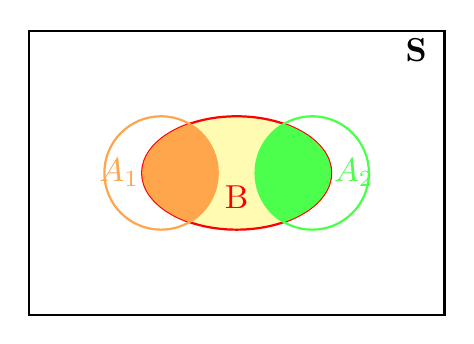
\begin{tikzpicture}[scale=1.2, every node/.style={transform shape}]
                    \draw[thick] (-2.2,-1.5) rectangle (2.2,1.5);
                    \node at (1.9, 1.3) {\textbf{S}};

                    % New sample space B
                    \fill[yellow!30] (0,0) ellipse (1cm and 0.6cm);
                    \draw[thick, red] (0,0) ellipse (1cm and 0.6cm) node[below] {B};

                    % Mutually exclusive events A1 and A2
                    \draw[thick, orange!70] (-0.8, 0) circle (0.6cm) node [left,xshift=-0.1cm] {\(A_1\)};
                    \draw[thick, green!70] (0.8, 0) circle (0.6cm) node[right,xshift=0.1cm] {\(A_2\)};
                    
                    % Color the intersections
                    \begin{scope}
                        \clip (0,0) ellipse (1cm and 0.6cm);
                        \fill[orange!70] (-0.8, 0) circle (0.6cm);
                        \fill[green!70] (0.8, 0) circle (0.6cm);
                    \end{scope}
                \end{tikzpicture}
            \end{block}
        \end{column}
    \end{columns}
\end{frame}

\subsubsection{Law of Total Probability}
\begin{frame} \vfill \centering \begin{beamercolorbox}[sep=10pt,center,shadow=false,rounded=true]{section_begin} \usebeamerfont{section_begin}\insertsubsubsectionhead\par \end{beamercolorbox} \vfill \end{frame}
\begin{frame}[t]
\vspace{-2mm}
\footnotesize
\frametitle{Partition of the Sample Space}
  \begin{Definisi}[Partition]
    A \textbf{partition} is a way to \textbf{break down or divide} the entire sample space ($S$) into several events (sets) $B_1, B_2, \dots, B_m$ that satisfy these conditions:
    \begin{enumerate}
        \item \textbf{Mutually Exclusive:} There is no intersection or overlap between the parts. An outcome cannot be in two parts at once. ($B_i \cap B_j = \emptyset$ for $i \neq j$)
        \item \textbf{Collectively Exhaustive:} If all parts are combined, they form the entire sample space again. ($B_1 \cup B_2 \cup \dots \cup B_m = S$)
    \end{enumerate}
  \end{Definisi}
\vspace{-1mm}
  \begin{exampleblock}{Intuitive Analogy}
      Imagine the sample space is a \textbf{whole cake}. A partition is when you \textbf{cut the cake} into several slices. Each slice is a $B_i$.
      \begin{itemize}
          \item The cake slices do not overlap (mutually exclusive).
          \item All the slices put back together make the whole cake (collectively exhaustive).
      \end{itemize}
      \end{exampleblock}
\end{frame}

\begin{frame}
\frametitle{\ }
  \vspace{-7mm}
  \footnotesize
  \begin{Teorema}[Event in a Partition][teorema:representasiperistiwadenganpartisi]
    Given a partition $\{B_1, B_2, \dots\}$ of the sample space and any event $A$. If we define new "pieces" $C_i = A \cap B_i$, then:
    \begin{enumerate}
        \item The pieces $C_i$ and $C_j$ are \textbf{mutually exclusive}.
        \item The union of all these pieces \textbf{reconstructs the event A} completely.
    \end{enumerate}
    \[
        A = C_1 \cup C_2 \cup \dots = (A \cap B_1) \cup (A \cap B_2) \cup \dots
    \]
  \end{Teorema}
  \only<1>{
\vspace{-7mm}
  \begin{block}{}
    \begin{itemize}
        \item \textbf{Sample Space (S)}: The entire map of a country.
        \item \textbf{Partition (B)}: The set of all regions (Region X, Region Y, Region Z, etc.). Each region is a $B_i$. They do not overlap and cover the entire country.
        \item \textbf{Event (A)}: The "Protected Forest Area" in the country. This area is spread across various regions.
    \end{itemize}
    
    This theorem states that the "Total Protected Forest Area" ($A$) can be seen as the union of: "Protected Forest Area \textbf{in} Region X" ($A \cap B_1$), "Protected Forest Area \textbf{in} Region Y" ($A \cap B_2$), and so on. Clearly, these specific areas are separate from one another.
    
  \end{block}
}
\only<2>{
  \begin{alertblock}{Why is This Theorem Important?}
    This theorem is a logical "stepping stone". It provides the mathematical justification that we are \textbf{allowed} to break down the probability $P[A]$ into the sum of the probabilities of its pieces, i.e., $\sum P[A \cap B_i]$, which is the core of the Law of Total Probability.
  \end{alertblock}
  }
\end{frame}

% --- NEW SLIDE 1: Theorem of Event in a Partition ---
\begin{frame}
    \frametitle{Theorem: Events in a Partition}
    
    \begin{columns}[T]
        \begin{column}{0.5\textwidth}
            \begin{block}{Theorem}
                Given a partition $\{B_1, B_2, \dots\}$ of the sample space and any event $A$. If we define new "pieces" $C_i = A \cap B_i$, then:
                \begin{enumerate}
                    \item The pieces $C_i$ and $C_j$ are \textbf{mutually exclusive}.
                    \item The union of all these pieces will \textbf{reconstruct the event A} completely.
                \end{enumerate}
                 \[ A = (A \cap B_1) \cup (A \cap B_2) \cup \dots \]
            \end{block}
        \end{column}
        
        \begin{column}{0.5\textwidth}
            \begin{block}{Illustration}
                \centering
                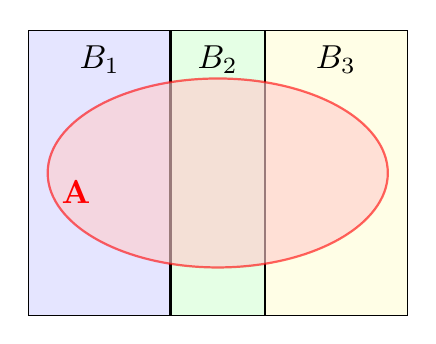
\begin{tikzpicture}[scale=1.2, every node/.style={transform shape}]
                    % Partition
                    \draw[thick] (-2,-1.5) rectangle (2,1.5);
                    \node at (1.7, 1.3) {\textbf{S}};
                    \fill[blue!10] (-2,-1.5) rectangle (-0.5,1.5);
                    \fill[green!10] (-0.5,-1.5) rectangle (0.5,1.5);
                    \fill[yellow!10] (0.5,-1.5) rectangle (2,1.5);
                    \draw[thick] (-0.5, -1.5) -- (-0.5, 1.5);
                    \draw[thick] (0.5, -1.5) -- (0.5, 1.5);
                    \node at (-1.25, 1.2) {\(B_1\)};
                    \node at (0, 1.2) {\(B_2\)};
                    \node at (1.25, 1.2) {\(B_3\)};
                    
                    % Event A
                    \draw[thick, red, fill=red!20, opacity=0.6] (0,0) ellipse (1.8cm and 1cm);
                    \node[red] at (-1.5, -0.2) {\textbf{A}};
                \end{tikzpicture}
            \end{block}
        \end{column}
    \end{columns}
\end{frame}

% --- NEW SLIDE 2: Visualization of the Theorem ---
\begin{frame}
    \frametitle{Visualizing the Theorem of Events in a Partition}
    
    \begin{columns}[T]
        \begin{column}{0.5\textwidth}
            \begin{block}{Explanation of Properties}
                \begin{enumerate}
                    \item \textbf{Mutually Exclusive}: Since \(B_1, B_2, \dots\) do not overlap, the pieces \(C_1, C_2, \dots\) which are parts of them cannot possibly overlap either.
                    \item \textbf{Forms A}: Every part of A must be located within one of the partition areas (e.g., \(B_i\)). Therefore, the union of all intersections (\(A \cap B_i\)) will cover all of A.
                \end{enumerate}
            \end{block}
        \end{column}
        
        \begin{column}{0.5\textwidth}
            \begin{block}{The Pieces \(C_i = A \cap B_i\)}
                \centering
                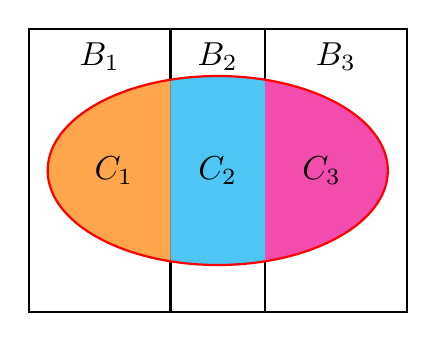
\begin{tikzpicture}[scale=1.2, every node/.style={transform shape}]
                    % Partition (lines only)
                    \draw[thick] (-2,-1.5) rectangle (2,1.5);
                    \draw[thick] (-0.5, -1.5) -- (-0.5, 1.5);
                    \draw[thick] (0.5, -1.5) -- (0.5, 1.5);
                    \node at (-1.25, 1.2) {\(B_1\)};
                    \node at (0, 1.2) {\(B_2\)};
                    \node at (1.25, 1.2) {\(B_3\)};
                    
                    % Color the pieces C_i
                    \begin{scope} % C1 = A intersect B1
                        \clip (-2,-1.5) rectangle (-0.5,1.5);
                        \fill[orange!70] (0,0) ellipse (1.8cm and 1cm);
                    \end{scope}
                    \begin{scope} % C2 = A intersect B2
                        \clip (-0.5,-1.5) rectangle (0.5,1.5);
                        \fill[cyan!70] (0,0) ellipse (1.8cm and 1cm);
                    \end{scope}
                    \begin{scope} % C3 = A intersect B3
                        \clip (0.5,-1.5) rectangle (2,1.5);
                        \fill[magenta!70] (0,0) ellipse (1.8cm and 1cm);
                    \end{scope}
                    
                    % Draw outline of A
                    \draw[thick, red] (0,0) ellipse (1.8cm and 1cm);
                    
                    % Label the pieces
                    \node at (-1.1, 0) {\(C_1\)};
                    \node at (0, 0) {\(C_2\)};
                    \node at (1.1, 0) {\(C_3\)};
                \end{tikzpicture}
            \end{block}
        \end{column}
    \end{columns}
\end{frame}

\begin{frame}[t]
\frametitle{\ }

    \begin{block}{Breaking Down Event A Using a Partition}
        Now imagine there is another event, $A$, within the sample space (e.g., "the part of the cake that has a cherry on it"). We can view this event $A$ through the "lens" of our partition. We can break down event $A$ into smaller pieces, namely the intersection of $A$ with each part of the partition: $C_i = A \cap B_i$. These pieces $C_i$ are guaranteed to be mutually exclusive.
    \end{block}
\end{frame}

\begin{frame}[t]
\frametitle{\ }
    \begin{Teorema}[Law of Total Probability (First Form)]
    \label{teorema:hukumprobabilitastotal1}
      For any event $A$ and a partition $\{B_1, \dots, B_m\}$, the probability of $A$ is:
      \[
        P[A] = \sum_{i=1}^{m} P[A \cap B_i]
      \]
    \end{Teorema}

    \begin{alertblock}{Intuitive Description}
      To find the total probability of event $A$, we can calculate the probability of the "piece of A" that is inside $B_1$, then the probability of the "piece of A" inside $B_2$, and so on, and then \textbf{sum them all up}.
    \end{alertblock}
\end{frame}

\begin{frame}
    \frametitle{Law of Total Probability}
    
    \begin{columns}[T]
        \begin{column}{0.5\textwidth}
            \begin{block}{Theorem}
      For any event $A$ and a partition $\{B_1, \dots, B_m\}$, the probability of $A$ is:
      \[
        P[A] = \sum_{i=1}^{m} P[A \cap B_i]
      \]
            \end{block}
            
            \begin{block}{Diagram Explanation}
                The total probability of A (the area of A) is the sum of the probabilities of its constituent "pieces".
            \end{block}
        \end{column}
        
        \begin{column}{0.5\textwidth}
            \begin{block}{Diagram: \(P[A] = \sum P[A \cap B_i]\)}
                \centering
                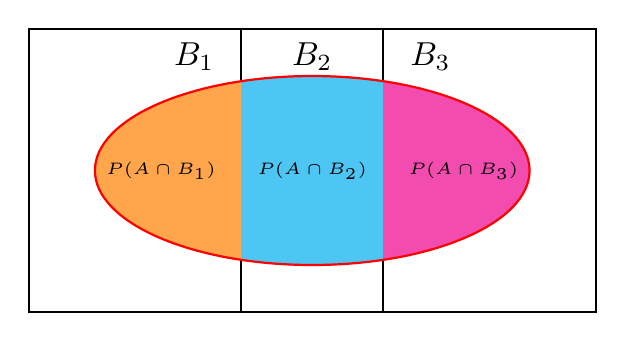
\begin{tikzpicture}[scale=1.2, every node/.style={transform shape}]
                    % Partition (lines only)
                    \draw[thick] (-3,-1.5) rectangle (3,1.5);
                    \draw[thick] (-0.75, -1.5) -- (-0.75, 1.5);
                    \draw[thick] (0.75, -1.5) -- (0.75, 1.5);
                    \node at (-1.25, 1.2) {\(B_1\)};
                    \node at (0, 1.2) {\(B_2\)};
                    \node at (1.25, 1.2) {\(B_3\)};
                    
                    % Color the pieces C_i
                    \begin{scope}
                        \clip (0,0) ellipse (2.3cm and 1cm);
                        \fill[orange!70] (-3,-1.5) rectangle (-0.75,1.5);
                        \fill[cyan!70] (-0.75,-1.5) rectangle (0.75,1.5);
                        \fill[magenta!70] (0.75,-1.5) rectangle (3,1.5);
                    \end{scope}
                    
                    \draw[thick, red] (0,0) ellipse (2.3cm and 1cm);
                    
                    % Labels
                    \node at (-1.6, 0) {\tiny \(P(A \cap B_1)\)};
                    \node at (0, 0) {\tiny \(P(A \cap B_2)\)};
                    \node at (1.6, 0) {\tiny \(P(A \cap B_3)\)};
                \end{tikzpicture}
            \end{block}
        \end{column}
    \end{columns}
\end{frame}

\begin{frame}[t]
\frametitle{\ }
    \begin{block}{Connecting with Conditional Probability}
        The previous form ($P[A \cap B_i]$) is sometimes difficult to calculate directly. We can change it using the definition of conditional probability:
        \[ P[A \cap B_i] = P[A|B_i] P[B_i] \]
        By substituting this into the previous theorem, we get the most common and useful form.
    \end{block}
\end{frame}

\begin{frame}[t]
\frametitle{\ }
\vspace{-7mm}
\footnotesize
    \begin{Teorema}[Law of Total Probability]
        For a partition $\{B_1, B_2, \dots, B_m\}$ with $P[B_i] > 0$ for all $i$, the probability of event $A$ is:
        \[
        P[A] = \sum_{i=1}^{m} P[A|B_i] P[B_i]
        \]
    \end{Teorema}

    \begin{exampleblock}{Intuitive Description and Usefulness}
     This is a \textbf{weighted average}. The total probability $P[A]$ is calculated by:
     \begin{enumerate}
         \item Taking the probability of $A$ occurring \textit{given that} we know we are in partition $B_i$ ($P[A|B_i]$).
         \item Multiplying (weighting) it by the probability that we are indeed in that partition $B_i$ ($P[B_i]$).
         \item Doing this for all parts of the partition, then summing the results.
     \end{enumerate}
     This is very useful when it's easier to know the probability of an event in \textbf{various scenarios/conditions} (the partition $B_i$) than to calculate it as a whole.
    \end{exampleblock}
\end{frame}

% --- NEW SLIDE 1: Law of Total Probability ---
\begin{frame}
    \frametitle{Law of Total Probability}
    
    \begin{columns}[T]
        \begin{column}{0.5\textwidth}
            \begin{block}{Theorem}
                For a partition $\{B_1, B_2, \dots, B_m\}$, the probability of event $A$ is:
                \[ P[A] = \sum_{i=1}^{m} P[A|B_i] P[B_i] \]
            \end{block}
            
            \begin{block}{Diagram Explanation}
                The total probability of A (the area of A) is the sum of the probabilities of its constituent "pieces".
                \vspace{0.5cm}
                
                Each piece, \(P(A \cap B_i)\), can be calculated as \(P(A|B_i)P(B_i)\). By summing all these pieces, we get the total probability of A.
            \end{block}
        \end{column}
        
        \begin{column}{0.5\textwidth}
            \begin{block}{Diagram: \(P[A] = \sum P[A|B_i]P[B_i]\)}
                \centering
                \begin{tikzpicture}[scale=1.2, every node/.style={transform shape}]
                    % Partition (lines only)
                    \draw[thick] (-3,-1.5) rectangle (3,1.5);
                    \draw[thick] (-0.75, -1.5) -- (-0.75, 1.5);
                    \draw[thick] (0.75, -1.5) -- (0.75, 1.5);
                    \node at (-1.25, 1.2) {\(B_1\)};
                    \node at (0, 1.2) {\(B_2\)};
                    \node at (1.25, 1.2) {\(B_3\)};
                    
                    % Color pieces C_i
                    \begin{scope}
                        \clip (0,0) ellipse (2.3cm and 1cm);
                        \fill[orange!70] (-3,-1.5) rectangle (-0.75,1.5);
                        \fill[cyan!70] (-0.75,-1.5) rectangle (0.75,1.5);
                        \fill[magenta!70] (0.75,-1.5) rectangle (3,1.5);
                    \end{scope}
                    
                    \draw[thick, red] (0,0) ellipse (2.3cm and 1cm);
                    
                    % Labels
                    \node at (-1.6, 0) {\tiny \only<1>{\(P(A \cap B_1)\)}\only<2>{\(P[A|B_1] P[B_1]\)}};
                    \node at (0, 0) {\tiny \only<1>{\(P(A \cap B_2)\)}\only<2>{\(P[A|B_2] P[B_2]\)}};
                    \node at (1.6, 0) {\tiny \only<1>{\(P(A \cap B_3)\)}\only<2>{\(P[A|B_3] P[B_3]\)}};
                \end{tikzpicture}
            \end{block}
        \end{column}
    \end{columns}
\end{frame}

\subsubsection{Bayes' Theorem}
\begin{frame} \vfill \centering \begin{beamercolorbox}[sep=10pt,center,shadow=false,rounded=true]{section_begin} \usebeamerfont{section_begin}\insertsubsubsectionhead\par \end{beamercolorbox} \vfill \end{frame}
\begin{frame}
\frametitle{\ }
\vspace{-7mm}
\footnotesize
  \begin{Teorema}[Bayes' Theorem][thm:bayes]
    If we have information about the conditional probability $P[A|B]$, we can calculate its "inverse", $P[B|A]$, using the following formula:
    \[
      P[B|A] = \frac{P[A|B] P[B]}{P[A]}
    \]
  \end{Teorema}

  \begin{block}{Intuitive Description: Updating Beliefs}
    Think of Bayes' Theorem as a mathematical way to \textbf{update our beliefs after getting new evidence}.
    \begin{itemize}
        \item $P[B]$: \textbf{Prior Belief}. How much you believe $B$ is true \textit{before} seeing new evidence.
        \item $P[A|B]$: \textbf{Likelihood}. How likely the evidence $A$ is to appear, \textit{if} your prior belief ($B$) is true.
        \item $P[A]$: \textbf{Probability of Evidence}. How common the evidence $A$ is in general, across all possibilities.
        \item $P[B|A]$: \textbf{Posterior Belief}. How much you believe $B$ is true \textit{after} seeing the evidence $A$.
    \end{itemize}
  \end{block}
\end{frame}

% --- NEW SLIDE: Bayes' Theorem ---
\begin{frame}
    \frametitle{\ }
    \vspace{-7mm}
    \begin{columns}[T]
        \begin{column}{0.5\textwidth}
            \begin{block}{Theorem}
                If we have information about the conditional probability $P[A|B]$, we can calculate its "inverse", $P[B|A]$, using the following formula:
                \[
                  P[B|A] = \frac{P[A|B] P[B]}{P[A]}
                \]
            \end{block}
        \end{column}
        
        \begin{column}{0.5\textwidth}
            \begin{block}{Diagram}
                \centering
                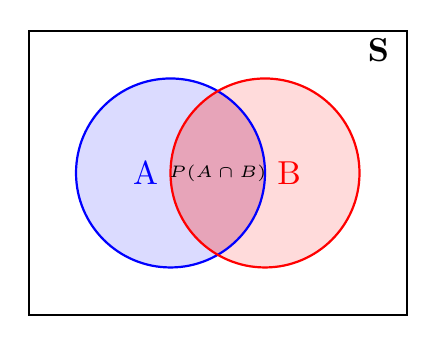
\begin{tikzpicture}[scale=1.2, every node/.style={transform shape}]
                    \draw[thick] (-2,-1.5) rectangle (2,1.5);
                    \node at (1.7, 1.3) {\textbf{S}};
                    
                    % Areas P(A) and P(B)
                    \fill[blue!20, opacity=0.7] (-0.5,0) circle (1cm);
                    \fill[red!20, opacity=0.7] (0.5,0) circle (1cm);
                    
                    % Intersection Area P(A intersect B)
                    \begin{scope}
                        \clip (-0.5,0) circle (1cm);
                        \fill[purple!40, opacity=0.8] (0.5,0) circle (1cm);
                    \end{scope}
                    
                    % Outlines
                    \draw[thick, blue] (-0.5,0) circle (1cm) node[left] {A};
                    \draw[thick, red] (0.5,0) circle (1cm) node[right] {B};
                    
                    % Label
                    \node at (0,0) {\tiny \(P(A \cap B)\)};
                \end{tikzpicture}
            \end{block}
        \end{column}
    \end{columns}
    \vspace{-1mm}
    \begin{block}{Diagram Explanation}
        Bayes' Theorem connects two conditional probabilities. Both depend on the \textbf{same intersection area} (\(P(A \cap B)\)), but are normalized by different sample spaces.
        \begin{itemize}
            \item \(P(A|B)\) uses B as its sample space.
            \item \(P(B|A)\) uses A as its sample space.
        \end{itemize}
    \end{block}
\end{frame}

\begin{frame}
    \frametitle{Visualizing Prior to Posterior}
    \setbeamertemplate{enumerate items}[default]
    \begin{columns}[T]
        \begin{column}{0.5\textwidth}
            \begin{block}{Diagram Explanation}
                \begin{enumerate}
                    \item \textbf{Prior}: The sample space is partitioned by hypotheses \(B_1\) and \(B_2\). Their areas represent our initial beliefs, \(P(B_1)\) and \(P(B_2)\).
                    \item \textbf{Evidence}: We observe new evidence, event A (the red area).
                    \item \textbf{Posterior}: After knowing A has occurred, our sample space shrinks to A. The posterior probability \(P(B_1|A)\) is the proportion of area A that came from \(B_1\), which is \(\frac{P(B_1 \cap A)}{P(A)}\).
                \end{enumerate}
            \end{block}
        \end{column}
        
        \begin{column}{0.5\textwidth}
            \begin{block}{Diagram: From \(P(B)\) to \(P(B|A)\)}
                \centering
                \begin{tikzpicture}[scale=1.2, every node/.style={transform shape}]
                    % Partition B1, B2
                    \only<1>{
                    \fill[blue!10] (-2,-1.5) rectangle (0,1.5);
                    \fill[green!10] (0,-1.5) rectangle (2,1.5);
                    }
                    \draw[thick] (-2,-1.5) rectangle (2,1.5);
                    \only<1>{
                    \node at (-1, 1.2) {\scriptsize \(P(B_1)\) (Prior)};
                    \node at (1, 1.2) {\scriptsize\(P(B_2)\) (Prior)};
                    }
                    % Evidence A
                    \only<1>{
                    \draw[thick, red, opacity=0.7] (0,0) ellipse (1.5cm and 1.0cm);
                    }
                    \only<2>{
                    \begin{scope}
                        \clip (0,0) ellipse (1.5cm and 1.0cm);
                        \fill[blue!10] (-2,-1.5) rectangle (0,1.5);
                        \fill[green!10] (0,-1.5) rectangle (2,1.5);
                        \draw[thick, red] (0,0) ellipse (1.5cm and 1.0cm);
                    \end{scope}
                    }
                    \fill[red, opacity=0.2] (0,0) ellipse (1.5cm and 1.0cm);
                    \node[red] at (1.1, 0.5) {A};
                    \only<2>{
                    % Labels
                    \node[align=center, scale=0.7](b1post) at (-0.7,0) {\(P(B_1 | A)\)};
                    \node[align=center, scale=0.7] at (0.7,0) {\(P(B_2 | A)\)};
                    }
                    
                    \only<2>{
                    \node[align=center, scale=0.7, yshift=-0.4cm, xshift=-0.9cm]{\scriptsize(Posterior)};
                    \node[align=center, scale=0.7, yshift=-0.4cm, xshift=0.9cm]{\scriptsize(Posterior)};
                    }

                    \draw[thick] (0,-1.5) -- (0,1.5);
                    \node at (-1.75,0.0) {\textbf{\(B_1\)}};
                    \node at (1.75,0.0) {\textbf{\(B_2\)}};
                    \node at (1.8,-1.2) {\textbf{S}};
                \end{tikzpicture}
            \end{block}
        \end{column}
    \end{columns}
\end{frame}

\begin{frame}
\frametitle{\ }
\vspace{-7mm}
\footnotesize
  \begin{exampleblock}{Classic Example: Medical Test}
    A rare disease affects 1\% of the population ($P[\text{Disease}] = 0.01$). A test exists with the following details:
    \begin{itemize}
        \item If you have the disease, the test is 99\% accurate in showing a positive result ($P[\text{Positive}|\text{Disease}] = 0.99$).
        \item If you are healthy, the test incorrectly shows a positive result 5\% of the time (false positive) ($P[\text{Positive}|\text{Healthy}] = 0.05$).
    \end{itemize}
    \textbf{Question:} If you receive a \textbf{positive} test result, what is the probability you actually have the disease? We are looking for $P[\text{Disease}|\text{Positive}]$.
    
    \medskip
    
    Using Bayes' Theorem:
    $P[\text{Disease}|\text{Positive}] = \frac{P[\text{Positive}|\text{Disease}] P[\text{Disease}]}{P[\text{Positive}]}$
    
    We calculate $P[\text{Positive}]$ with the Law of Total Probability:
    $P[\text{Positive}] = (0.99 \times 0.01) + (0.05 \times 0.99) = 0.0594$
    
    Therefore, $P[\text{Disease}|\text{Positive}] = \frac{0.99 \times 0.01}{0.0594} \approx 0.1667$ or \textbf{only 16.67\%!}

    \medskip
    
    \textbf{Intuitive Conclusion:} Even though the test is very accurate, because the disease is so rare (low prior belief), a positive result is more likely to be a false positive from the much larger healthy population.
  \end{exampleblock}
\end{frame}

\subsubsection{Independent Events}
\begin{frame} \vfill \centering \begin{beamercolorbox}[sep=10pt,center,shadow=false,rounded=true]{section_begin} \usebeamerfont{section_begin}\insertsubsubsectionhead\par \end{beamercolorbox} \vfill \end{frame}
\begin{frame}[t]
\frametitle{\ }
\vspace{-9mm}
\only<1>{
    \begin{Definisi}[Two Events]
        A and B are independent if $P[A \cap B] = P[A]P[B]$.
        \begin{itemize}
            \item \textbf{When to Use:} When the outcome of one event provides no information about the outcome of another.
            \item \textbf{Example Meaning:} The probability of getting Heads on a coin AND a 6 on a die is $P(H) \times P(6) = 1/2 \times 1/6$.
        \end{itemize}
    \end{Definisi}
}
\only<2>{
    \begin{Definisi}[Three Events]
        Events A, B, and C are mutually independent if \textbf{all} of the following conditions are met:
        \begin{itemize}
            \item $P[A \cap B] = P[A]P[B]$
            \item $P[A \cap C] = P[A]P[C]$
            \item $P[B \cap C] = P[B]P[C]$
            \item $P[A \cap B \cap C] = P[A]P[B]P[C]$
        \end{itemize}
        \begin{itemize}
            \item \textbf{When to Use:} To model systems with many independent components (e.g., 3 coin flips). It is not enough to just check the intersection of all three.
            \item \textbf{Example Meaning:} The probability of getting (Heads, Heads, Heads) on 3 fair coin flips is $P(H_1 \cap H_2 \cap H_3) = P(H_1)P(H_2)P(H_3) = \frac{1}{2}\times\frac{1}{2}\times\frac{1}{2} = \frac{1}{8}$.
        \end{itemize}
    \end{Definisi}
}

\only<3>{
\begin{Definisi}[More Than Two Independent Events]
    If $n \ge 3$, the events $A_1, A_2, \dots, A_n$ are \textbf{mutually independent} if and only if
    \begin{itemize}
        \item[(a)] any collection of $n-1$ events chosen from $A_1, A_2, \dots, A_n$ is mutually independent,
        \item[(b)] $P[A_1 \cap A_2 \cap \dots \cap A_n] = P[A_1]P[A_2]\cdots P[A_n]$.
    \end{itemize}
\end{Definisi}
}
\end{frame}

\begin{frame}
    \frametitle{\ }
    \footnotesize
    \vspace{-8mm}
    \begin{columns}[T]
        \begin{column}{0.5\textwidth}
            \begin{block}{Definition}
                Two events A and B are called independent if the occurrence of A does not affect the probability of B occurring. Mathematically:
                \[ P(A \cap B) = P(A)P(B) \]
            \end{block}
            \vspace{-4mm}
            \begin{block}{Common Misconception}
                \begin{itemize}
                    \item \textbf{Independent vs. Mutually Exclusive}: These are two different concepts. Mutually exclusive (\(A \cap B = \emptyset\)) means both events cannot happen at the same time. Independent means the occurrence of one event does not change the probability of the other.
                \end{itemize}
            \end{block}
        \end{column}
        
        \begin{column}{0.5\textwidth}
            \begin{block}{Intersecting Diagram}
                \centering
                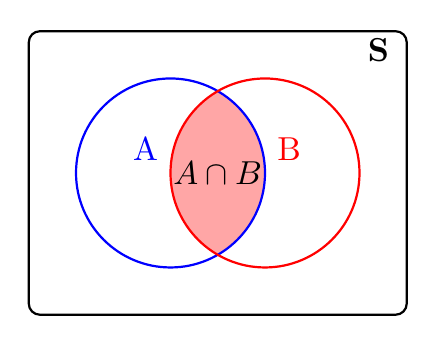
\begin{tikzpicture}[scale=1.2, every node/.style={transform shape}]
                    \draw[thick, rounded corners] (-2,-1.5) rectangle (2,1.5);
                    \node at (1.7, 1.3) {\textbf{S}};
                    
                    \begin{scope}
                        \clip (-0.5,0) circle (1cm);
                        \fill[red!50, opacity=0.7] (0.5,0) circle (1cm);
                    \end{scope}
                    
                    \draw[thick, blue] (-0.5,0) circle (1cm) node[above left] {A};
                    \draw[thick, red] (0.5,0) circle (1cm) node[above right] {B};
                    
                    \node at (0,0) {\(A \cap B\)};
                \end{tikzpicture}
            \end{block}
            \vspace{-0.5mm}
            \begin{block}{Venn Diagram Intuition}
            \begin{itemize}
                \item The existence of an intersection (\(A \cap B \neq \emptyset\)) is actually a \textit{requirement} for two events (with probability > 0) to be independent. If they were mutually exclusive, then \(P(A \cap B)=0\), which would not equal \(P(A)P(B)\) unless one of the probabilities was zero.
            \end{itemize}
            \end{block}
        \end{column}
    \end{columns}
\end{frame}

% --- SLIDE 17: Example of Independent but Intersecting ---
\begin{frame}
    \frametitle{\ }
    \vspace{-7mm}
    \footnotesize
    \begin{columns}[T]
        \begin{column}{0.5\textwidth}
            \begin{block}{Experiment: Rolling Two Dice}
                \begin{itemize}
                    \item \textbf{A}: The first die shows a 3. \\ \(P(A) = 6/36 = 1/6\).
                    \item \textbf{B}: The sum of the two dice is 7. \\ \(B = \{(1,6), (2,5), (3,4), (4,3), (5,2), (6,1)\}\). \\ \(P(B) = 6/36 = 1/6\).
                    \item \textbf{Intersection \(A \cap B\)}: The first die is 3 AND the sum is 7. This is only possible if the outcome is \{(3,4)\}. \\ \(P(A \cap B) = 1/36\).
                \end{itemize}
            \end{block}
            \vspace{-4mm}
            \begin{block}{Proof}
                Is \(P(A \cap B) = P(A)P(B)\)?
                \[ \frac{1}{36} = \frac{1}{6} \times \frac{1}{6} \]
                Yes, it is true. Therefore, A and B are \textbf{independent despite having an intersection.}
            \end{block}
        \end{column}
        
        \begin{column}{0.5\textwidth}
            \begin{block}{Diagram Still Intersects}
                \centering
                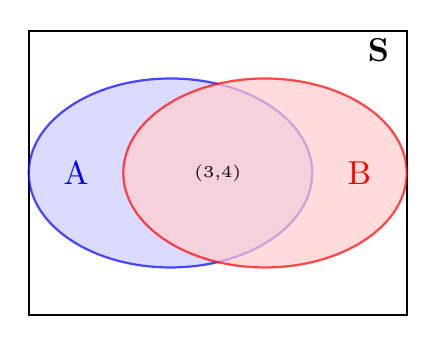
\begin{tikzpicture}[scale=1.2, every node/.style={transform shape}]
                    \draw[thick] (-2,-1.5) rectangle (2,1.5);
                    \node at (1.7, 1.3) {\textbf{S}};
                    
                    % A and B
                    \draw[thick, blue, fill=blue!20,opacity=0.7] (-0.5,0) ellipse (1.5cm and 1cm);
                    \node[blue] at (-1.5, 0) {A};
                    \draw[thick, red, fill=red!20,opacity=0.7] (0.5,0) ellipse (1.5cm and 1cm);
                    \node[red] at (1.5, 0) {B};
                    
                    % Intersection
                    \node at (0,0) {\tiny (3,4)};
                \end{tikzpicture}
            \end{block}
        \end{column}
    \end{columns}
\end{frame}

\subsubsection{Conditional Independence}
\begin{frame} \vfill \centering \begin{beamercolorbox}[sep=10pt,center,shadow=false,rounded=true]{section_begin} \usebeamerfont{section_begin}\insertsubsubsectionhead\par \end{beamercolorbox} \vfill \end{frame}

\begin{frame}[t]
\frametitle{Independence That Holds Inside One Group}
\vspace{1mm}
\footnotesize
\begin{Definisi}[Conditional Independence]
    Two events $A$ and $B$ are \textbf{conditionally independent given} $H$ if
    \[ P[A \cap B \mid H] = P[A \mid H]\, P[B \mid H], \]
    or equivalently, if $P[B \mid A, H] = P[B \mid H]$ whenever $P[A \mid H] > 0$.
\end{Definisi}
\vspace{-2mm}
\begin{itemize}\setlength\itemsep{2pt}
    \item Read it as: \emph{inside the group $H$}, learning that $A$ occurred does not change the probability of $B$.
    \item A comma inside the bar means ``and'': $P[B \mid A, H]$ is the probability of $B$ among the outcomes that satisfy $A$ \emph{and} $H$ at the same time.
    \item The condition must hold in \textbf{every} group. Independence given $H$ alone is not enough; $H^c$ has to be checked as well.
\end{itemize}
\end{frame}

\begin{frame}[t]
\frametitle{Two Kinds of Independence That Are Easily Confused}
\vspace{1mm}
\footnotesize
\begin{columns}[T]
    \begin{column}{0.48\textwidth}
        \begin{block}{Independence (unconditional)}
            \[ P[A \cap B] = P[A]P[B] \]
            Holds across the whole population, without separating any group.
        \end{block}
    \end{column}
    \begin{column}{0.48\textwidth}
        \begin{block}{Conditional independence}
            \[ P[A \cap B \mid H] = P[A \mid H]P[B \mid H] \]
            Holds inside the group $H$, once the group has been fixed first.
        \end{block}
    \end{column}
\end{columns}
\vspace{2mm}
\begin{alertblock}{Neither one implies the other}
    Two events can be independent inside every group and still look dependent once the groups are pooled --- and the other way round. That is why the two must be named separately, and never abbreviated to just ``independent''.
\end{alertblock}
\end{frame}

\begin{frame}[t]
\frametitle{Why the Assumption Is Tempting, and When It Fails}
\vspace{1mm}
\footnotesize
\begin{block}{The temptation}
    If $A$ and $B$ are taken to be conditionally independent given $H$, the probability that both occur is just a product:
    \[ P[A \cap B \mid H] = P[A \mid H]\,P[B \mid H]. \]
    One multiplication, with nothing new to measure. That is why the assumption is used everywhere, often without ever being stated.
\end{block}
\vspace{-1mm}
\begin{block}{When it fails}
    When a \textbf{common cause} drives $A$ and $B$ together. Once $A$ is known to have occurred, that cause becomes more likely to be present, so $B$ becomes more likely too --- \emph{even with the group already fixed}. In symbols: $P[B \mid A, H] \neq P[B \mid H]$.
\end{block}
\vspace{-1mm}
\begin{itemize}
    \item The way to check is not intuition but data: measure $P[B \mid H]$ and $P[B \mid A, H]$, then compare. Equal, and the assumption may be used; different, and it may not.
    \item The same check must be repeated on $H^c$. That is often where the gap is widest.
\end{itemize}
\end{frame}

\subsection{Guided Case-Study Quiz Example}
\begin{frame} \vfill \centering \begin{beamercolorbox}[sep=10pt,center,shadow=false,rounded=true]{section_begin} \usebeamerfont{section_begin}\insertsubsectionhead\par \end{beamercolorbox} \vfill \end{frame}

\begin{frame}[t]
\frametitle{What It Looks Like}
\vspace{1mm}\footnotesize
From Week 2 onwards, every synchronous session closes with a Guided Case-Study Quiz. The example below uses Week 1 material so that its shape is visible before the real one arrives.
\begin{block}{What makes a quiz ``guided''}
\begin{itemize}\setlength\itemsep{1pt}
    \item The case is presented by the lecturer in that same session, so there is nothing to memorise beforehand.
    \item The working is \emph{scaffolded}: the table is already drawn, and you only fill in the cells.
    \item Every answer is a number or a tick box --- nothing depends on how you word a sentence.
    \item Graded automatically on EMAS3. Each quiz is worth 4\%, eight times across the semester.
\end{itemize}
\end{block}
\begin{alertblock}{What is being trained here}
Not speed, but the habit of counting before concluding. The weight per quiz is deliberately small so that you are allowed to be slow and unsure without paying much for it.
\end{alertblock}
\end{frame}

\begin{frame}[t]
\frametitle{The Case and Its Archive Figures}
\vspace{1mm}\footnotesize
A system reviews one complete interview session and then raises two flags: a \emph{language flag} and a \emph{voice flag}. What the officer actually wants to know --- whether the applicant's account is problematic --- cannot be observed directly.
\vspace{1mm}
\begin{center}\scriptsize
\begin{tabular}{|c|l|c|l|}
\hline
$H$ & account is problematic & $H^c$ & account is not problematic \\ \hline
$A$ & language flag up & $A^c$ & language flag not up \\ \hline
$B$ & voice flag up & $B^c$ & voice flag not up \\ \hline
\end{tabular}
\vspace{2mm}

\begin{tabular}{|l|c|c|}
\hline
\textbf{Quantity} & \textbf{Symbol} & \textbf{Value} \\ \hline
Sessions whose account is problematic & $P(H)$ & $0.04$ \\ \hline
Language flag up, among problematic sessions & $P(A \mid H)$ & $0.50$ \\ \hline
Language flag up, among unproblematic sessions & $P(A \mid H^c)$ & $0.10$ \\ \hline
\end{tabular}
\end{center}
\vspace{1mm}
Imagine $10{,}000$ sessions.
\end{frame}

\begin{frame}[t]
\frametitle{The Question --- Exactly as You Will Receive It}
\vspace{1mm}\footnotesize
A new officer says: \emph{``The language flag is up in half of all problematic sessions, so if the flag is up, the chance this session is problematic is about 50\%.''} Check that.
\vspace{2mm}

\textbf{(a)} Complete the table: two empty cells under \textbf{Number of sessions}, then three under \textbf{Flagged sessions}.
\begin{center}\scriptsize
\begin{tabular}{|l|c|c|c|}
\hline
\textbf{Group} & \textbf{Number of sessions} & \textbf{Probability flag is up} & \textbf{Flagged sessions} \\ \hline
Problematic & \underline{\hspace{1.4cm}} & $0.50$ & \underline{\hspace{1.4cm}} \\ \hline
Unproblematic & \underline{\hspace{1.4cm}} & $0.10$ & \underline{\hspace{1.4cm}} \\ \hline
\textbf{Total} & $10{,}000$ & \textemdash & \underline{\hspace{1.4cm}} \\ \hline
\end{tabular}
\end{center}
\vspace{1mm}
\textbf{(b)} From that table, what fraction of the flagged sessions is problematic? State it as a percentage to two decimal places.
\vspace{1mm}

\textbf{(c)} Tick the name of the theorem that assembles the ``Total'' row: \quad $\square$~Bayes' theorem \quad $\square$~law of total probability \quad $\square$~probability axioms
\end{frame}

\begin{frame}[t]
\frametitle{Worked Solution}
\vspace{1mm}\footnotesize
\textbf{(a)} From $P(H) = 0.04$: problematic $10{,}000 \times 0.04 = 400$, unproblematic $9{,}600$.
\begin{center}\scriptsize
\begin{tabular}{|l|c|c|c|}
\hline
\textbf{Group} & \textbf{Number of sessions} & \textbf{Probability flag is up} & \textbf{Flagged sessions} \\ \hline
Problematic & $\mathbf{400}$ & $0.50$ & $\mathbf{200}$ \\ \hline
Unproblematic & $\mathbf{9{,}600}$ & $0.10$ & $\mathbf{960}$ \\ \hline
\textbf{Total} & $10{,}000$ & \textemdash & $\mathbf{1{,}160}$ \\ \hline
\end{tabular}
\end{center}
\vspace{1mm}
\textbf{(b)} $P(H \mid A) = 200/1{,}160 = \mathbf{17.24\%}$. The officer is wrong, and off by almost a factor of three.
\vspace{1mm}

\textbf{(c)} \textbf{Law of total probability} --- the ``Total'' row is assembled by sweeping across both groups, $200 + 960$. Bayes' theorem only does its work in step (b), when the numerator is divided by that total.
\vspace{1mm}
\begin{alertblock}{Why the gap is that wide}
Not because the flag is bad. Unproblematic sessions are far more numerous, so $9{,}600 \times 0.10 = 960$ false alarms drown out the $200$ correct detections. Even a detector that caught \emph{every} problematic session would still face those $960$.
\end{alertblock}
\end{frame}

\begin{frame}[t]
\frametitle{The Rest of It, and Where the Full File Lives}
\vspace{1mm}\footnotesize
The complete example has four questions. The one just worked through is question 1; the other three continue with the same case:
\begin{itemize}\setlength\itemsep{2pt}
    \item \textbf{Question 2} --- the voice flag is brought in as well. Two ways of computing give different answers ($29.41\%$ and $20.00\%$); an archive note decides which one applies. What is being tested: the conditional independence assumption.
    \item \textbf{Question 3} --- a four-state table produced by manual review. What is being tested: partitioning the sample space, and which flag actually carries information.
    \item \textbf{Question 4} --- matching each step already carried out with the name of the theory behind it.
\end{itemize}
\vspace{1mm}
\begin{block}{Files}
The full version, with all solutions and the mark breakdown, is on EMAS3: \textbf{Guided-Case-Study-Quiz-Week1}. Two companion files sit alongside it --- a sample Case-Study Quiz (unguided) and a Midterm specimen --- so that the difference between the three kinds of question can be seen side by side.
\end{block}
\end{frame}

\subsection{Q\&A}
\begin{frame}
\frametitle{Q\&A}
\vspace{-5mm}
    \begin{center}
        \Huge Any Questions?
    \end{center}
\end{frame}

\section{Conclusion}
\subsection{Summary}
\SetSlideHeaderLevel{section}
\begin{frame}[t]
\frametitle{Basic Definitions \& Terms}
    \begin{block}{Key Points}
        Probability is a formal way to measure and talk about uncertainty. We use specific terms to avoid ambiguity.
        \begin{itemize}
            \item \textbf{Experiment}: The procedure we observe.
            \item \textbf{Outcome}: A single possible result.
            \item \textbf{Sample Space ($S$)}: The collection of \textit{all} possible outcomes.
            \item \textbf{Event}: A collection of one or more outcomes that we are interested in.
        \end{itemize}
    \end{block}
\end{frame}

\begin{frame}[t]
\frametitle{Set Operations \& Boolean Logic}
    \begin{block}{Key Points}
        Set theory provides the "grammar" for probability, allowing us to combine and manipulate events.
        \begin{itemize}
            \item \textbf{Intersection ($A \cap B$)} is logical \textbf{AND}: The event where A \textit{and} B both occur.
            \item \textbf{Union ($A \cup B$)} is logical \textbf{OR}: The event where A \textit{or} B (or both) occur.
            \item \textbf{Complement ($A^c$)} is logical \textbf{NOT}: The event where A does \textit{not} occur.
        \end{itemize}
    \end{block}
\end{frame}

\begin{frame}[t]
\frametitle{Axioms of Probability}
    \begin{block}{The Three Basic Rules}
        All probability calculations, no matter how complex, must adhere to these three fundamental rules:
        \begin{enumerate}
            \item \textbf{Non-negativity:} $P(A) \ge 0$. Probability cannot be negative.
            \item \textbf{Total Certainty:} $P(S) = 1$. Something from all possibilities must happen.
            \item \textbf{Addition for Mutually Exclusive Events:} If A and B cannot happen together, $P(A \cup B) = P(A) + P(B)$.
        \end{enumerate}
    \end{block}
\end{frame}

\begin{frame}[t]
\frametitle{Theorems of Probability}
    \begin{block}{Key Points}
        Using the axioms as a foundation, we can derive theorems that become our everyday tools.
        \begin{itemize}
            \item \textbf{Complement Rule:} $P(A^c) = 1 - P(A)$. A quick way to calculate the probability of "not A".
            \item \textbf{General Addition Rule:} $P(A \cup B) = P(A) + P(B) - P(A \cap B)$. This formula corrects for double-counting in events that can overlap.
            \item \textbf{Probability from Outcomes:} $P(B) = \sum P(s_i)$. The probability of an event is the sum of the probabilities of each outcome within it.
        \end{itemize}
    \end{block}
\end{frame}

\begin{frame}[t]
\frametitle{Conditional Probability}
    \begin{block}{Key Points}
        Conditional probability, $P(A|B)$, answers the question: "What is the probability of A, \textit{given that we already know} that B has occurred?"
        \[ P(A|B) = \frac{P(A \cap B)}{P(B)} \]
        This effectively "shrinks" our sample space from $S$ to just $B$.
    \end{block}
\end{frame}

\begin{frame}[t]
\frametitle{Law of Total Probability \& Bayes' Theorem}
    \begin{block}{Two Powerful Tools}
        \begin{itemize}
            \item \textbf{Law of Total Probability}: Allows us to calculate the probability of an event ($A$) by breaking it down based on several possible scenarios (a partition $B_i$). It's a "divide and conquer" strategy.
            \item \textbf{Bayes' Theorem}: Uses the result from the Law of Total Probability to reverse the condition. If we know $P(A|B)$, Bayes' Theorem helps us find $P(B|A)$.
        \end{itemize}
    \end{block}
\end{frame}

\begin{frame}[t]
\frametitle{Independence}
    \frametitle{Summary: When Events Do Not Influence Each Other}
    \begin{block}{Key Definition}
        Two events A and B are said to be \textbf{independent} if the occurrence of one does not change the probability of the other occurring. Mathematically:
        \[ P(A \cap B) = P(A) \times P(B) \]
        This is a very powerful simplifying assumption.
    \end{block}
\end{frame}

\subsection{Upcoming Lecture}
\begin{frame}[t]
\frametitle{Upcoming Lecture}
\begin{alertblock}{Bridge to the Next Topic}
    Throughout this week every probability was computed over a single event that had already happened. Next week the question shifts: if an experiment is run repeatedly or in stages, how many ways can its outcomes be arranged, and what is the probability of each arrangement? That is where \textbf{sequential experiments} and their counting rules --- permutations, combinations, and the multinomial coefficient --- come in as the tools for computing it.
\end{alertblock}
\end{frame}

\subsection{Q\&A}
\begin{frame}[fragile]
\frametitle{Q\&A Session}
    \begin{center}
        \Huge Thank You
        \vspace{2cm}
        
        Questions?
    \end{center}
\end{frame}